\section{Implementación del lazo cerrado}
\subsection{Variable controlada y referencia}
Se conserva la planta termoeléctrica de la Tarea 1, con corriente $I$ como entrada y temperatura $T_b$ del bloque frío como salida. Se adopta como objetivo nominal $T_b=5\,{}^\circ\mathrm C$, ambiente de $25\,{}^\circ\mathrm C$ y flujo de aire de $400\,\mathrm{LFM}$. El punto de operación guardado en el proyecto es
\begin{align}
 I_0&=1.190149\,\mathrm A, &T_{b0}&=278.15\,\mathrm K,\\
 T_{h0}&=304.101077\,\mathrm K, &R_{HA}&=1.29\,\mathrm{K/W}.
\end{align}
La referencia representa regulación de una carga térmica, por lo que resulta físicamente coherente con la salida modelada. Para estudiar el seguimiento local se propone un cambio de $5$ a $4\,{}^\circ\mathrm C$ en $t=20\,\mathrm s$. El arranque se estudia por separado, con ambas masas inicialmente a $25\,{}^\circ\mathrm C$ y referencia constante de $5\,{}^\circ\mathrm C$; esta condición está alejada de la linealización.

\subsection{Convención de signo y límites}
Como la ganancia de pequeña señal de la planta es negativa, se define
\begin{align}
 e(t)&=T_{b,\mathrm{med}}(t)-T_{\mathrm{ref}}(t),\\
 I(t)&=\operatorname{sat}_{[0,\,6.4]}\{I_0+K_p e(t)\}.
\end{align}
Una temperatura superior a la referencia produce un incremento de corriente para $K_p>0$. El sesgo $I_0$ mantiene la corriente necesaria en el equilibrio nominal. La planta física recibe corriente absoluta; la representación lineal recibe $\Delta I=I-I_0$. Las temperaturas internas se expresan en kelvin y se convierten a grados Celsius para la medición y las figuras.

\begin{figure}[!tbp]
\centering
\begin{tikzpicture}[>=Latex,font=\scriptsize,
 b/.style={draw,align=center,minimum height=8mm,inner sep=3pt}]
\node[draw,circle,inner sep=2pt] (e) at (0,0) {$\Sigma$};
\node[b] (k) at (1.35,0) {$K_p$};
\node[b] (s) at (3.0,0) {$+I_0$\\Saturación};
\node[b] (p) at (5.2,0) {Planta\\$I\mapsto T_b$};
\node (y) at (6.5,0) {};
\draw[->] (e)--node[above]{$e$}(k);
\draw[->] (k)--(s);
\draw[->] (s)--node[above]{$I$}(p);
\draw[->] (p)--node[above]{$T_b$}(y.center);
\draw[->] (6.2,0)--(6.2,-1.0)--node[below]{$T_b+n$}(0,-1.0)--node[left]{$+$}(e);
\draw[->] (-0.9,0.65)node[above]{$T_{\rm ref}$}--(-0.9,0)--node[above]{$-$}(e);
\draw[->] (5.2,0.9)node[above]{$Q_{\rm carga}$}--(p);
\end{tikzpicture}
\caption{Lazo de acción inversa. El ruido $n$ se suma en la medición; la perturbación térmica entra en la planta.}
\label{fig:lazoP}
\end{figure}

La implementación propuesta utiliza dos modelos. La red Simscape se reutiliza de la Tarea 1. En la representación lineal se conservan los dos estados térmicos para incorporar condiciones iniciales, una entrada adicional de calor y la temperatura caliente. Una rama con la función de transferencia $G(s)$ verifica la salida de pequeña señal desde equilibrio. Así se mantiene el mismo modelo lineal de la tarea previa y se evita atribuir a una función de transferencia con condiciones iniciales nulas un arranque que no describe por sí sola.

\section{Análisis del controlador proporcional}
La función de transferencia nominal es
\begin{equation}
G(s)=\frac{-0.291898s-0.00424337}{s^2+0.0563263s+0.000410735}.
\end{equation}
Sin saturación, la transferencia de referencia a salida y el polinomio característico son
\begin{align}
 T_P(s)&=\frac{-K_pG(s)}{1-K_pG(s)},\\
 D_P(s)&=s^2+(0.0563263+0.291898K_p)s\notag\\
 &\quad +(0.000410735+0.00424337K_p).
\end{align}
Los coeficientes son positivos para $K_p>0$ y el criterio de segundo orden establece estabilidad del modelo lineal nominal. Esta conclusión es local: no demuestra regulación global con saturación ni con variaciones grandes de temperatura.

Para un escalón de referencia de magnitud $|\Delta r|$, la magnitud del error estacionario lineal es
\begin{equation}
 |e_{ss}|=\frac{|\Delta r|}{1-K_pG(0)}\simeq\frac{|\Delta r|}{1+10.331K_p}.
\end{equation}
El error que usa el controlador es $T_b-T_{\rm ref}$; en las tablas se reporta también su magnitud para facilitar la comparación. La fórmula anterior corresponde a un cambio de referencia respecto del equilibrio. En un arranque que retorna al punto nominal, el sesgo $I_0$ puede permitir error final cero si el sistema converge y no recibe perturbaciones constantes.

\begin{table}[!tbp]\centering
\caption{Cálculo lineal nominal para un escalón de $1\,\mathrm K$.}
\label{tab:teoriaP}
\footnotesize
\begin{tabular}{@{}cccc@{}}\toprule
$K_p$ [A/K]&Polo 1 [s$^{-1}$]&Polo 2 [s$^{-1}$]&$|e_{ss}|$ [K]\\\midrule
0.2&$-0.102408$&$-0.012298$&0.32613\\
1&$-0.334302$&$-0.013922$&0.08825\\
5&$-1.501410$&$-0.014405$&0.01899\\\bottomrule
\end{tabular}
\end{table}
El aumento de ganancia reduce el error, pero uno de los polos se aproxima al cero de la planta, situado cerca de $-0.01454\,\mathrm{s}^{-1}$. Deben examinarse tanto su posición como la amplitud de su contribución a la salida: un tiempo de subida corto no excluye una cola lenta.

En el arranque, el mando inicial solicitado es $I_0+20K_p$. Para las ganancias estudiadas se obtienen $5.190$, $21.190$ y $101.190\,\mathrm A$; las dos últimas quedan limitadas a $6.4\,\mathrm A$. El calentamiento Joule y el aumento de temperatura del disipador hacen necesario contrastar el arranque lineal con la planta no lineal.

\section{Evaluación del desempeño}
\subsection{Pruebas y métricas}
Se prepararon cuatro pruebas de $1200\,\mathrm s$ para ambas plantas y $K_p=0.2$, $1$ y $5\,\mathrm{A/K}$: escalón de referencia, arranque desde ambiente, carga de calor de $2\,\mathrm W$ desde $300\,\mathrm s$ y ruido de medición desde ese mismo instante. La carga y el ruido se aplican en ensayos separados. El ruido tiene desviación estándar elegida de $0.05\,\mathrm K$ y muestras mantenidas durante $1\,\mathrm s$; representa una condición comparativa, no un sensor medido.

La función \texttt{metricas\_lazo.m} evalúa error, tiempo de subida, establecimiento, sobrepaso, corriente máxima, tiempo en saturación e ISE. Se usa temperatura real para el error de seguimiento. El tiempo de subida corresponde al 10--90\% del cambio final alcanzado y solo se interpreta si el movimiento es en el sentido solicitado y la cola se estabiliza.

Se distinguen establecimiento respecto de la referencia y estabilización alrededor del valor final estimado. La banda del primero es $0.02\,\mathrm K$ para el escalón de $1\,\mathrm K$ y $0.4\,\mathrm K$ para el arranque de $20\,\mathrm K$. Si no se observa permanencia hasta el final de la simulación, el establecimiento se reporta como no alcanzado. Para la perturbación se usa una banda comparativa de $0.02\,\mathrm K$, pendiente de contrastar con las especificaciones definitivas del grupo.

El valor final se estima promediando el último 10\% del intervalo evaluado. Si el rango de temperatura en esa ventana supera la banda, el código no presenta ese promedio como un error estacionario. La ausencia de variación observada no se considera una demostración formal de estabilidad.

\subsection{Comprobación auxiliar de las ecuaciones}
\textbf{Los siguientes valores proceden de integración independiente en Python, no de ejecución en MATLAB/Simulink.} Se incluyen para contrastar la implementación posterior. El residuo del equilibrio nominal fue inferior a $10^{-13}\,\mathrm{K/s}$ y los errores del escalón lineal coincidieron con la fórmula de ganancia DC dentro de $2\times10^{-5}\,\mathrm K$.

\begin{table}[!tbp]\centering
\caption{Predicción auxiliar no lineal, pendiente de validar en Simscape. Magnitud del error en régimen observado.}
\label{tab:auxiliarP}
\footnotesize
\begin{tabular}{@{}ccc@{}}\toprule
$K_p$ [A/K]&Escalón de 1 K [K]&Carga de 2 W [K]\\\midrule
0.2&0.3331&1.7736\\
1&0.09184&0.5394\\
5&0.01990&0.1228\\\bottomrule
\end{tabular}
\end{table}
La predicción de arranque con $K_p=0.2\,\mathrm{A/K}$ se aproxima a la referencia y entra en la banda de $0.4\,\mathrm K$ alrededor de $252\,\mathrm s$. Con ganancias de $1$ y $5\,\mathrm{A/K}$, la integración predice enfriamiento inicial seguido de un aumento de temperatura y permanencia prolongada en el límite de corriente. Las temperaturas elevadas exceden el alcance confiable del modelo de coeficientes constantes; se interpretan como fallo del ensayo de regulación y no como predicción física precisa.

Este comportamiento sustenta revisar el tratamiento del arranque y los límites al diseñar el compensador. No basta añadir acción integral para afirmar que el problema desaparece; se debe verificar su implementación, incluido el anti-windup si corresponde.

\subsection{Resultados de la ejecución requerida}
\IfFileExists{../resultados_matlab/simscape_escalon.pdf}{%
\begin{figure}[!tbp]\centering
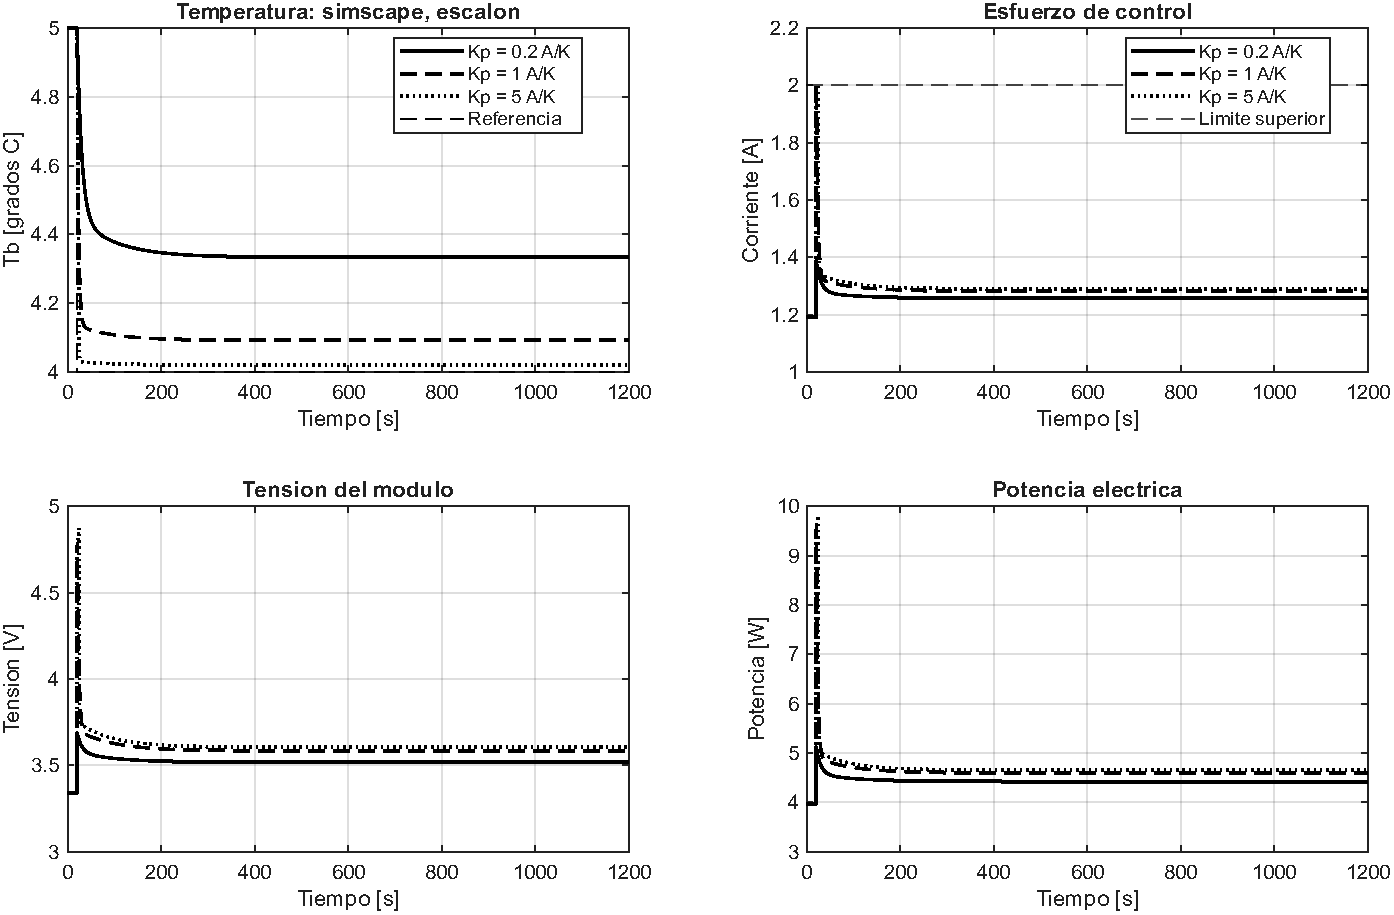
\includegraphics[width=\columnwidth]{../resultados_matlab/simscape_escalon.pdf}
\caption{Ensayo P de escalón, generado por la ejecución del modelo físico. Interpretar junto con \texttt{metricas\_P.csv}.}
\end{figure}
}{\textit{Pendiente: ejecutar los modelos nuevos en R2025a, verificar sus señales e incorporar las figuras y métricas realmente obtenidas.}}

La comparación definitiva debe incluir curvas de temperatura y corriente, las métricas y una interpretación por ensayo. El funcionamiento de los scripts y modelos nuevos no se certifica mediante la comprobación auxiliar.

\section{Sensibilidad paramétrica y limitaciones}
Se preparó la repetición del escalón nominal variando $R_{HA}$ entre $1.29$, $2.11$ y $8.4\,\mathrm{K/W}$, la masa fría en $\pm20\%$ y el punto de operación a $10\,{}^\circ\mathrm C$. Se mantienen las ganancias. Para el cambio de masa se conserva la resistencia térmica y se modifica la capacidad de almacenamiento; para el punto de $10\,{}^\circ\mathrm C$ se recalcula el sesgo de equilibrio de ambos controladores y se usa un escalón de $10$ a $9\,{}^\circ\mathrm C$.

Antes de atribuir diferencias al controlador se evaluó la factibilidad estática con los balances de la planta. Un barrido de corrientes de $0$ a $6.4\,\mathrm A$, con paso de $0.001\,\mathrm A$, produjo los mínimos aproximados de la Tabla~\ref{tab:factibilidad}. Se excluyeron equilibrios inestables y temperaturas absolutas no físicas.

\begin{table}[!tbp]\centering
\caption{Factibilidad calculada con el modelo térmico de Tarea 1.}
\label{tab:factibilidad}
\footnotesize
\begin{tabular}{@{}ccc@{}}\toprule
Disipación&$T_{b,\min}$ [$^\circ$C]&Corriente [A]\\\midrule
400 LFM&$-1.053$&2.421\\
200 LFM&6.710&1.681\\
Natural&20.146&0.495\\\bottomrule
\end{tabular}
\end{table}
Según estas hipótesis, $5\,{}^\circ\mathrm C$ no es un equilibrio alcanzable con 200 LFM ni con convección natural. Un compensador no elimina esta restricción física. En tales casos deben discutirse saturación, rechazo térmico y validez de las temperaturas predichas, en lugar de exigir cumplimiento de una referencia imposible.

El estudio P está programado y se dispone de una referencia auxiliar de las ecuaciones. La comparación compensada permanece condicionada a recibir la ley de control, sus parámetros y el modelo del integrante 3. Se prepararon los mismos casos y la unión de tablas, sin inventar ganancias ni presentar resultados compensados ausentes.

\section{Conclusiones parciales}
El control P reduce el error local al aumentar la ganancia, con los compromisos de esfuerzo y ruido que deben cuantificarse en las pruebas. La estabilidad lineal nominal no asegura el arranque del sistema físico saturado. La comprobación auxiliar advierte un fallo de arranque para las dos ganancias mayores, que debe contrastarse con Simscape. Además, la sensibilidad de la disipación revela límites de factibilidad que requieren distinguir el diseño de control del dimensionamiento térmico. El cierre de estas conclusiones exige la ejecución reproducible en R2025a y la comparación con el compensador real del grupo.
